\section{Introduction}
\begin{frame}{Motivation}
\begin{columns}
\column{0.5\textwidth}
\begin{itemize}
\item Many challenges exist regarding modern combustion systems 
\item Better modeling can improve performance, efficiency, and reliability 
\item Detonation engines are a growing area of interest 
\begin{itemize}
    \item Aircraft turbine propulsion
    \item Rocket aerospike-based propulsion
\end{itemize}
\item Current CFD models are computationally expensive
\item Adaptive meshing can reduce computational expense
\end{itemize}	

\column{0.5\textwidth}
\begin{figure}
\centering
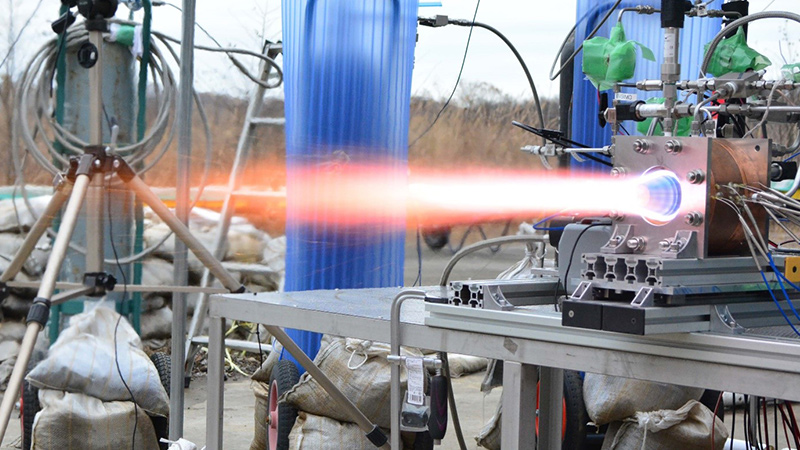
\includegraphics[width=\textwidth]{../figs/rde.jpg}
\caption{Nagoya University 900 N Rotating Detonation Engine \cite{nagoya}}
\end{figure}
\end{columns}
\end{frame}

\begin{frame}{Objectives}
\begin{itemize}
\item Implement and test AMR techniques for simulations of detonations found within RDEs and PDEs within OpenFOAM \cite{weller}, which has:
\begin{itemize}
\item geometric flexibility 
\item consistent input structure (easy to transition between solvers)
\item good documentation
\item open source, GNU GPL
\item industry use
\item existing infrastructure with the high-performance computing clusters used by TESLa
\end{itemize}
\item Build a framework on previous work by Towery \cite{towery1} and TESLa at CU Boulder for further RDE and PDE research 
\end{itemize}
\end{frame}

\begin{frame}{Previous Work}
\begin{itemize}
\item PDE and RDE numerical modeling on static grids 
\item Detonation modeling with AMR using in-house codes
\item Flame and combustion modeling with AMR in OpenFOAM
\item OpenFOAM detonation modeling with AMR without parallel computing or open source
\end{itemize}
\end{frame}

\begin{frame}{Previous Work: Towery \cite{towery1}}
\begin{columns}
\column{0.6\textwidth}
\begin{itemize}
\item Linear detonation tube modeling with in-house Fortran code
\item Compared numerical models to Chapman-Jouguet \cite{chapman} (CJ) detonation model
\item Able to produce ZND von Neumann pressure spike \cite{zeldovich,neumann,doring}
\item Simulated idealized and discrete injection, unrolled RDEs 
\end{itemize}
\column{0.4\textwidth}
\begin{center}
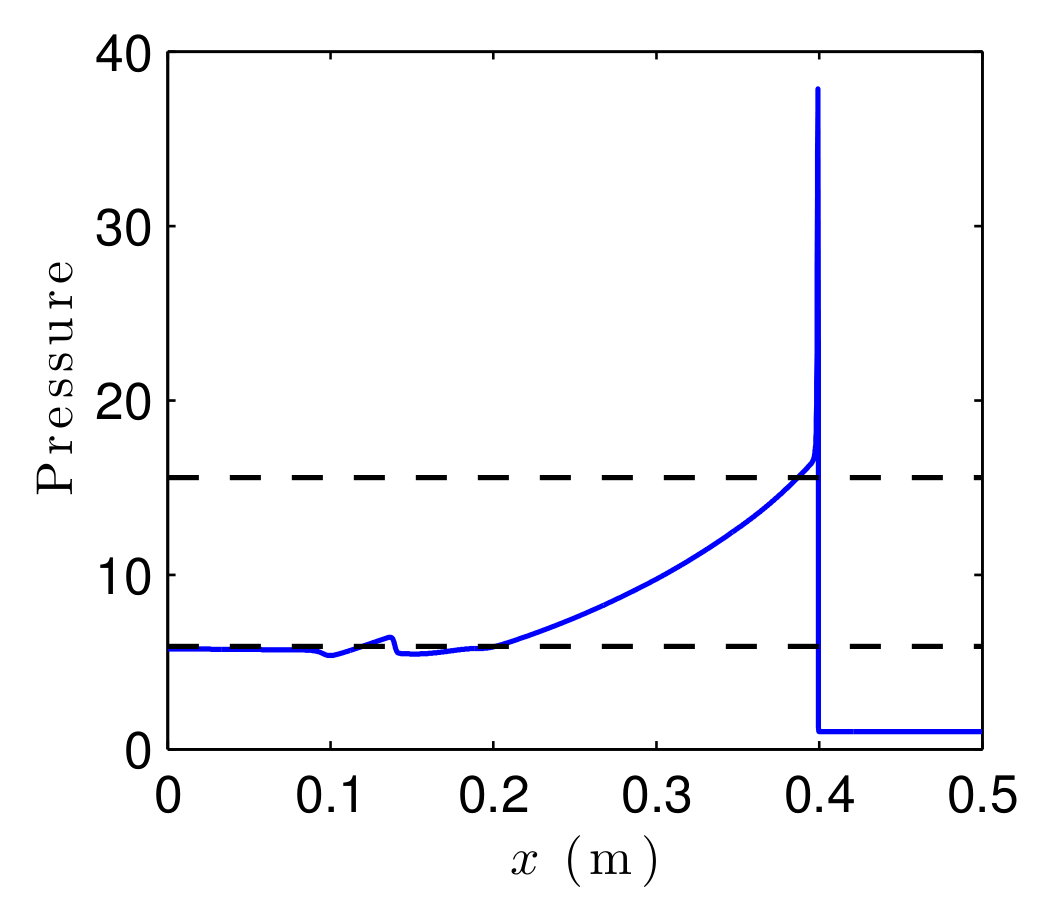
\includegraphics[width=\textwidth]{../figs/towery/pressure.png}    
\end{center}
\end{columns}    
\end{frame}

%\begin{frame}{Previous Work: Towery \cite{towery1} ii}
%
%\end{frame}


\begin{frame}{Solver Motivation}
Many combustion solvers exist, why do we need a {\color{red} new one}? 
\begin{table}
\begin{tabular}{|c|c|c|c|c|} \hline
Open-source & OpenFOAM & Detonations & Adaptive Meshing & Parallelized \\ \hline \hline
  & X & X &   & X \\ \hline
X & X & X &   & X \\ \hline
  & X & X & X &   \\ \hline
X & X & X &   & X \\ \hline
X &   & X & X & X \\ \hline
X & X &   & X & X \\ \hline
\color{red}{X} & \color{red}{X} & \color{red}{X} & \color{red}{X} & \color{red}{X} \\ \hline
\end{tabular}
\end{table}
\end{frame}
